\nsecbegin{JUnit}

JUnit ist ein Framework zum Testen von Java-Programmen, das besonders für automatisierte Unit-Tests einzelner Units (Klassen oder Methoden) geeignet ist.Die aktuelle Version ist JUnit 5, bestehend aus JUnit Platform, JUnitJupiter und JUnit Vintage.

In JUnit Jupiter werden die Tests geschrieben, in JUnit Platform ausgeführt und mit JUnit Vintage können ältere Versionen von JUnit - Junit 3 und JUnit4 - durchgeführt werden.

JUnit muss für die Nutzung in Eclipse nicht extra installiert werden, aber die JUnit 5 Library muss in den Build Path des jeweiligen Projektes aufgenommen werden. Von Eclipse gibt es auch eine Anleitung dazu 
%https://www.eclipse.org/eclipse/news/4.7.1a/#junit-5-support
\footnote{\url{https://www.eclipse.org/eclipse/news/4.7.1a/\#junit-5-support}}

Zuerst einmal wird das Projekt erstellt mit einem zusätzlichen Source-Ordner für den Test:
 %Bild1
\begin{figure}[H]
\centering
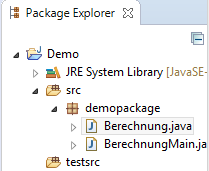
\includegraphics{Bilder/TRJU_1.png}
%\includegraphics[scale=•]{•}
\end{figure}
 
Mit Rechtsklick auf die Klasse, die getestet werden soll, kann ihr ein JUnit Test Case zugewiesen werden:
 %Bild2
 \begin{figure}[H]
\centering
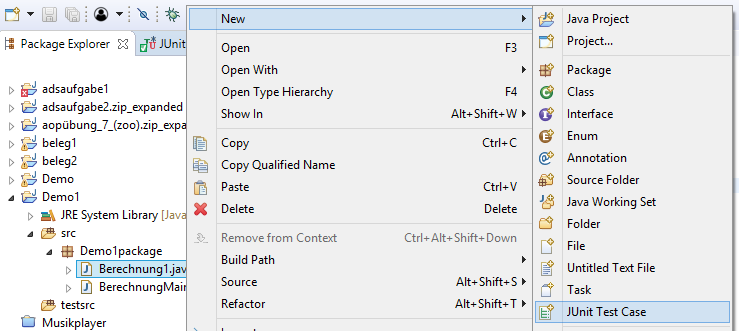
\includegraphics[width=\textwidth]{Bilder/TRJU_2.png}
%\includegraphics[scale=•]{•}
%\caption{Mit Rechtsklick auf die Klasse, die getestet werden soll, kann ihr ein JUnit Test Case zugewiesen werden}
\end{figure}

 Als Source-Folder wird dabei der dafür angelegte gewählt:
 %Bild3
 \begin{figure}[H]
\centering
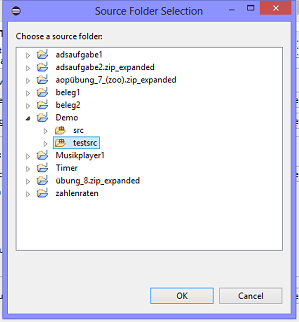
\includegraphics{Bilder/TRJU_3.png}
%\caption{Als Source-Folder wird dabei der dafür angelegte gewählt}
%\includegraphics[scale=•]{•}
\end{figure}

Anschließend klickt man auf die Schaltfläche Next > und kann auswählen, was getestet werden soll:  
%Bild4
\begin{figure}[H]
\centering
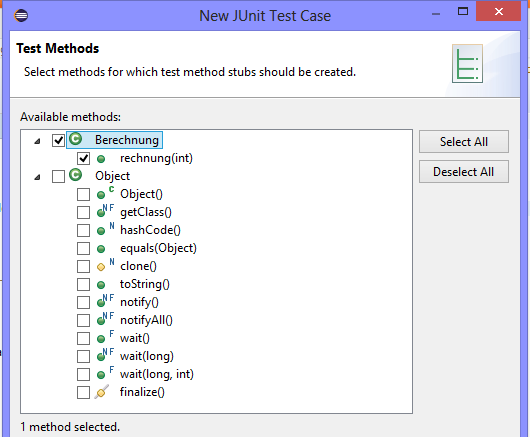
\includegraphics{Bilder/TRJU_4.png}
%\caption{Anschließend klickt man auf die Schaltfläche Next > und kann auswählen, was getestet werden soll}
%\includegraphics[scale=•]{•}
\end{figure}

Nach Klicken auf den Button Finish muss noch die JUnit 5 library zum Build Path hinzugefügt werden:
 %Bild5
 \begin{figure}[H]
\centering
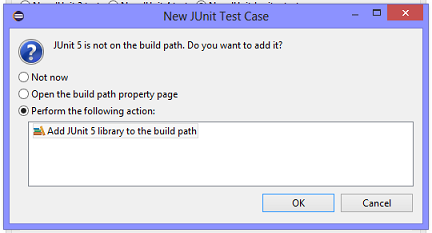
\includegraphics{Bilder/TRJU_5.png}
%\caption{Nach Klicken auf den Button Finish muss noch die JUnit 5 library zum Build Path hinzugefügt werden}
%\includegraphics[scale=•]{•}
\end{figure}
 Der automatisch erstellte Test kann jetzt  an das eigene Projekt angepasst werden. 
 In einem Test werden die Parameter (hier int a), das erwartete und die Berechnung des tatsächlichen Ergebnisses angegeben. Mit assertEquals(expected, actual); werden die beiden Ergebnisse miteinander verglichen. 
%Bild6
\begin{figure}[H]
\centering
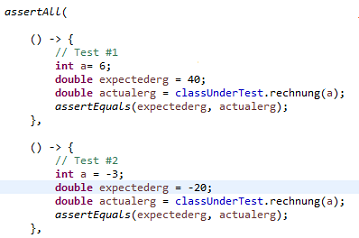
\includegraphics{Bilder/TRJU_6.png}
%\caption{Der automatisch erstellte Test kann jetzt  an das eigene Projekt angepasst werden.  In einem Test werden die Parameter (hier int a), das erwartete und die Berechnung des tatsächlichen Ergebnisses angegeben. Mit assertEquals(expected, actual); werden die beiden Ergebnisse miteinander verglichen. }
%\includegraphics[scale=•]{•}
\end{figure}

Mit dieser Anweisung kann festgelegt werden, dass eine Funktion vor jedem einzelnen Test durchgeführt werden. 
@BeforeEach
public void SetUp() throws Exception {
    classunderTest = new Berechnung();
}

Weitere Anweisungen wie diese sind zum Beispiel @BeforeAll (= bevor irgendein Test durchgeführt wird), @AfterEach (nach jedem Test)und  @AfterAll (nach allen Tests).

Nach Durchführung eines Testes erscheint links anstelle des Package Explorer ein JUnit Tab mit dem Ergebnis des Tests. 
 %Bild7
 \begin{figure}[H]
\centering
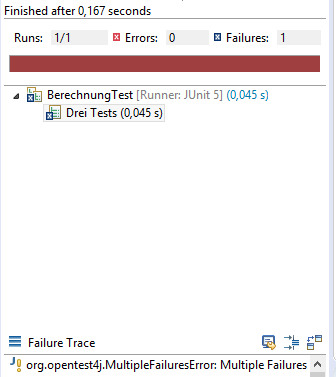
\includegraphics{Bilder/TRJU_7.png}
%\includegraphics[scale=•]{•}
%\caption{Nach Durchführung eines Testes erscheint links anstelle des Package Explorer ein JUnit Tab mit dem Ergebnis des Tests.Bei einem nicht bestandenen Test ist der Balken rot und unten wird klein angezeigt, warum der Test nicht bestanden wurde. Mit den drei Buttons rechts über dem Text kann man die Ansicht ändern (vlnr): Konsolenansicht, Filter Stack Trace (default), Side by Side comparison. Bei bestandenem Test ist der Balken grün.}
\end{figure}
Bei einem nicht bestandenen Test ist der Balken rot und unten wird klein angezeigt, warum der Test nicht bestanden wurde.

Mit den drei Buttons rechts über dem Text kann man die Ansicht ändern (vlnr): 
%Konsolenansicht, Filter Stack Trace (default), Side by Side comparison.

Bei bestandenem Test ist der Balken grün.

Ein etwas ausführlicheres Tutorial (auf Englisch) gibt es hier
\footnote{\url{https://www.youtube.com/watch?v=QNv_AQk6WWI}}
\nsecend %{JUnit}